\section{数据特征与公共物理模型}
\subsection{数据来源与统一口径}
\paragraph{（1）数据对象及其关联关系}
节点、货箱、运输机、中继机和通信参数分别由五份工作簿提供，地形由30米DEM描述\textsuperscript{\cite{Data2026}}。表\ref{tab:inputs}给出参与建模的对象规模。逐箱货箱清单作为分配的最小粒度，需求汇总表用于交叉核对；不能同时把两张表中的需求累加。
\begin{table}[htbp]\centering
\caption{标准场景的数据与资源构成}\label{tab:inputs}
\begin{tabularx}{\linewidth}{lYl}\toprule
对象 & 计算用途 & 规模\\\midrule
调度节点 & 航段、投送与网关定位 & 1个中心、15个服务区\\
逐箱需求 & 不可拆分配送与逐箱时限 & 80箱、53条汇总记录\\
运输无人机 & 机型选择与实体调度 & A/B/C共8架\\
运输电池 & 同型共享与充电周转 & A/B/C共14组\\
中继设备 & 空中接入与网关回传 & 2架、6组能源组件\\
DEM & 最高地形与视线遮挡 & $1309\times1486$像元\\
\bottomrule\end{tabularx}\end{table}

节点与需求空间关系见图\ref{fig:service-map}。点位决定飞行距离，点面积反映需求质量；二者共同影响组批，但尚不能据此判断某节点需要多少架次，因为安全载荷还受爬升和返航余量约束。
\begin{figure}[htbp]\centering
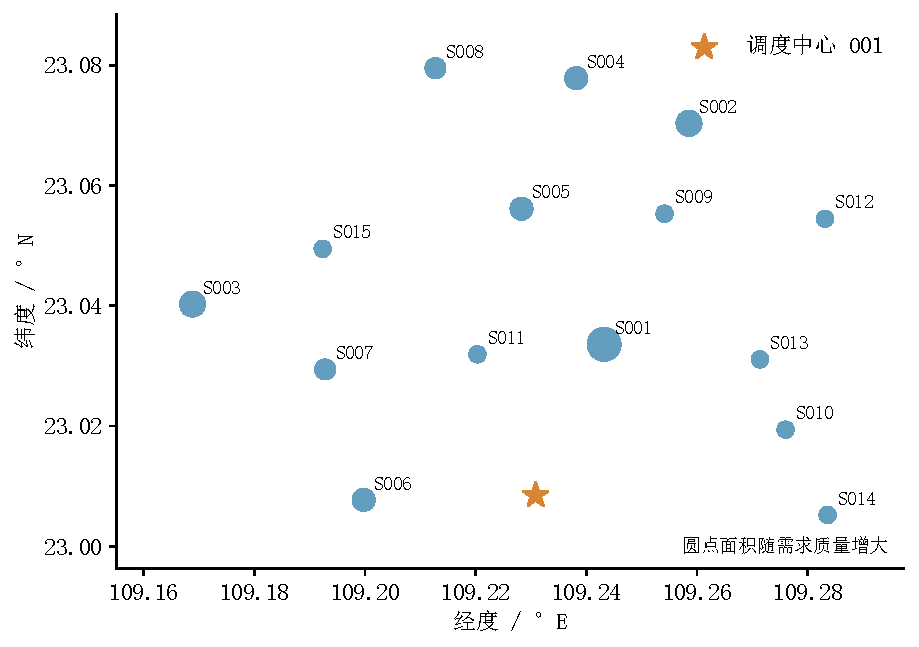
\includegraphics[width=.86\linewidth]{figures/data/raw_service_map.pdf}
\caption{调度中心与服务区分布：依据附件节点坐标与逐区需求绘制}
\label{fig:service-map}\end{figure}

\subsection{数据预处理与质量控制}
\paragraph{（1）编号、单位与缺失值处理}
不同附件以节点、货箱、机型和实体设备作为主键。预处理首先统一去除编号两端空格，保留前导零，并检查服务区编号是否属于S001--S015、中心与网关是否对应O01和G01。货箱目的地必须能在节点表中找到，实体无人机与电池必须能映射到A/B/C机型，中继能源组件则单独编号。任何无法建立外键关系的记录都不进入求解，而应回到原始附件核查。

质量统一为kg、体积统一为m$^3$、距离统一为m、时间内部统一为s、能量统一为kWh、功率统一为kW。经纬度仅用于空间定位，进入距离和DEM索引前转换为弧度或像元坐标；通信计算再把三维距离换算为km，以匹配自由空间损耗公式中的常数。单位转换在数据入口完成，避免在各子问题中重复换算产生口径漂移。

对关键字段执行非空和范围检查：货箱质量体积必须为正；机型容量、可用能量、速度和效率必须在物理允许范围内；SOC和安全余量位于$[0,1]$；中继离地高度不超过300~m。题目附件中的确定参数不采用均值填补。若关键值缺失，相关对象被标记为不可计算，而不是由相邻记录推测。

\paragraph{（2）需求汇总与双向核对}
逐箱清单是优化模型的权威需求源，因为不可拆货箱、类别、优先系数和时限均定义在箱级。需求汇总表只用于检查：按服务区聚合逐箱质量、体积和箱数后，应与汇总记录一致；再按物资类别核对医疗箱、首批保障箱及其交集。式\eqref{eq:hard-count}中的31箱来自集合并集，而不是简单相加。

求解输出也执行反向核对。问题一和问题二完成后，将结果表按货箱编号展开，要求原始80个编号与输出80个编号集合完全相同，且每个编号出现次数恰为1；按服务区重新汇总质量和体积，应回到输入值。该双向检查能够发现“总箱数正确但某箱重复、另一箱遗漏”的隐蔽错误。

\paragraph{（3）空间数据与DEM配准}
DEM栅格通过其经纬度范围和行列数建立地理坐标到像元索引的映射。由于栅格行方向通常与纬度增加方向相反，预处理需分别验证四角坐标和中心点索引，避免把南北方向翻转。节点若落在DEM范围外应立即报错；航段若穿越边界，则该路线不能直接按现有DEM证明净空。

固定步长采样可能跳过恰好位于两采样点之间的高程像元。本文除15~m密集采样外，计算航线与经纬向半像元边界的交点，再在相邻交点间取中点，从而枚举直线实际穿过的最近邻像元。对每一航段保存最高像元高程及其索引，既用于巡航海拔，也用于后续通信视线检查。

表\ref{tab:data-quality}汇总从编号关联、需求守恒到DEM配准和输出覆盖的主要质量控制规则，并说明各类异常会影响哪一层模型。
\begin{table}[htbp]\centering
\caption{数据质量控制规则及其对模型的影响}\label{tab:data-quality}
\small
\begin{tabularx}{\textwidth}{>{\raggedright\arraybackslash}p{2.7cm}YY}
\toprule
检查对象 & 质量控制规则 & 未通过时的影响\\
\midrule
节点与货箱编号 & 主键唯一；货箱目的地必须存在于节点表 & 无法完成任务归属，停止求解并核对附件\\
需求守恒 & 逐箱汇总与服务区汇总的箱数、质量、体积一致 & 不能用汇总表替代逐箱表，也不能重复累计\\
机型与实体资源 & 每架实体机和电池映射到唯一机型，数量与库存表一致 & 会造成错误的容量或并发资源上限\\
时间与单位 & 秒、小时、kg、m$^3$、kWh、kW在入口统一 & 会直接改变能耗、充电或截止判断\\
DEM范围与方向 & 节点在栅格内；四角与中心索引方向核对 & 会造成航段最高地形和视线遮挡错误\\
输出覆盖 & 80箱各出现一次，目的地和原始记录一致 & 发现遗漏、重复或错误交付即判方案无效\\
\bottomrule
\end{tabularx}\end{table}

\subsection{需求结构与时限分类}
\paragraph{（1）硬时限集合的构造}
逐箱统计得到总质量758 kg、总体积2.011 m$^3$。其中医疗箱16箱，首批保障箱30箱，二者交集15箱，故具有至少一种硬时限要求的货箱数为
\begin{equation}N_{hard}=16+30-15=31.\label{eq:hard-count}\end{equation}
余下49箱使用期望送达时间计算软迟到。交集不能重复计数：同一货箱既为医疗物资又为首批保障时，应取两个适用截止时刻的较小值，而不是将其视为两项配送任务。

\paragraph{（2）需求规模与紧迫性分布}
图\ref{fig:demand}同时展示需求质量和硬软时限构成。这一组合图把载荷规模与时间紧迫程度并列，便于识别“质量较大”与“必须尽早送达”并非同一概念。图\ref{fig:deadlines}进一步区分仅医疗、仅首批、两者兼有和一般物资；相同坐标的样本合并表示，避免重叠掩盖数量。

从逐区统计可见，S001拥有15箱、154 kg需求，约占总质量的20.3\%；S009至S015各有3箱、25 kg需求。S001的硬时限箱为3箱，其余服务区均为2箱，说明需求质量的差异明显大于硬时限箱数量的差异。调度时需要既给各区配置早期保障，又为大需求节点安排后续运力，不能仅按总质量大小排序服务。
\begin{figure}[htbp]\centering
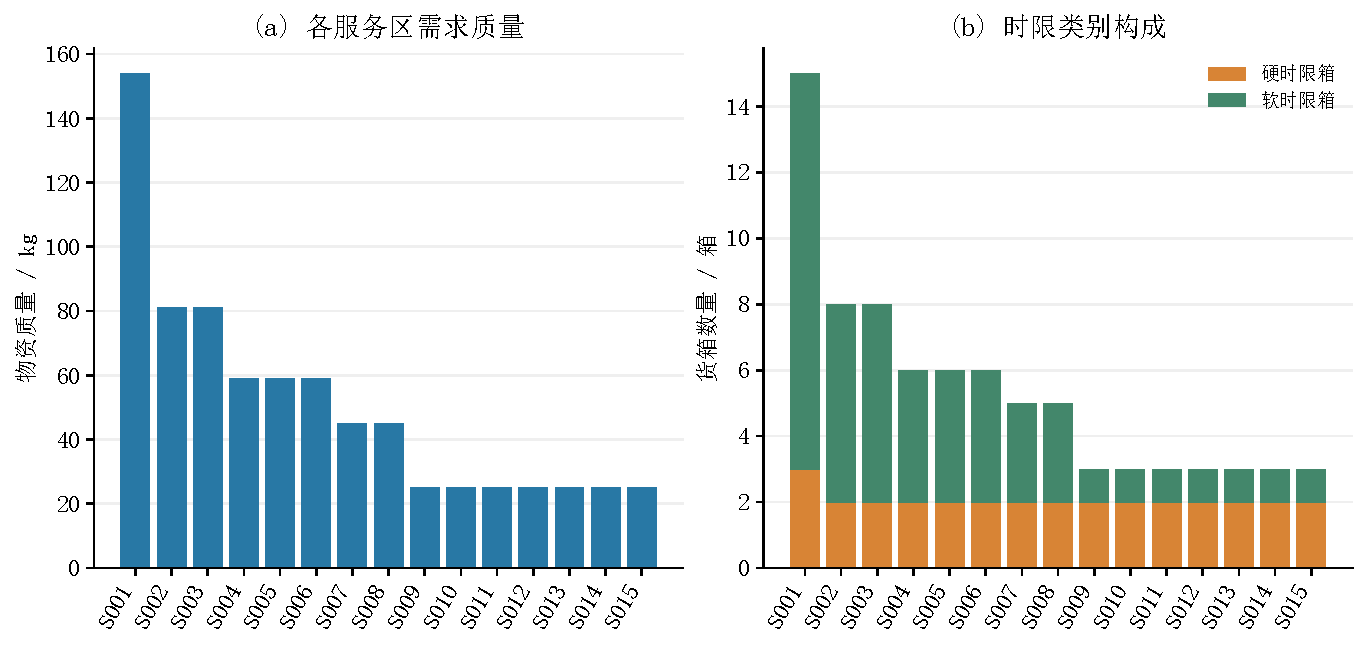
\includegraphics[width=\linewidth]{figures/data/raw_demand_composition.pdf}
\caption{各服务区的需求质量及硬软时限货箱构成}\label{fig:demand}\end{figure}
\begin{figure}[htbp]\centering
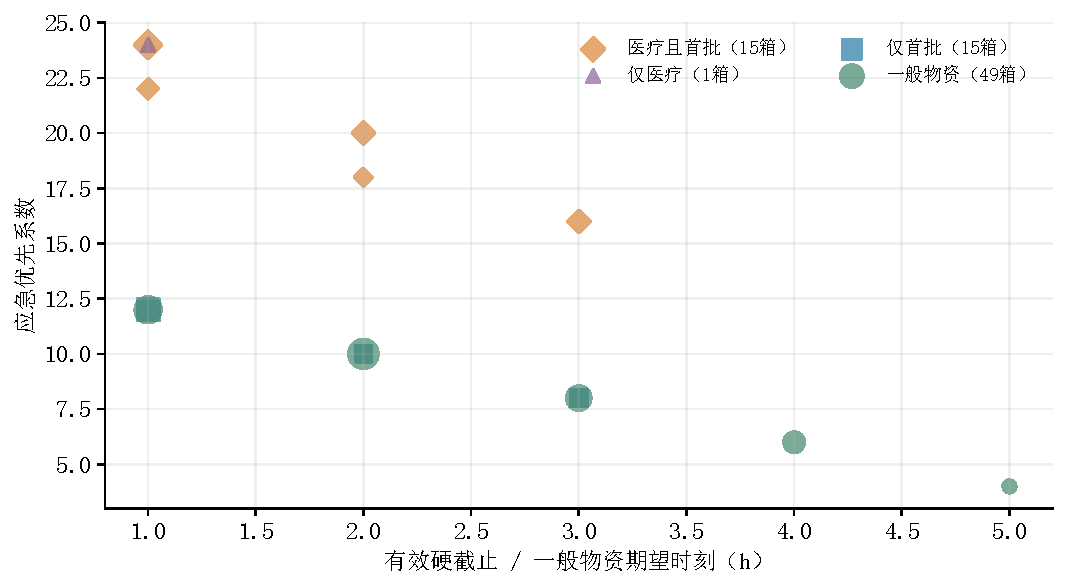
\includegraphics[width=.9\linewidth]{figures/data/raw_deadline_classes.pdf}
\caption{时限与优先系数：硬时限箱采用有效截止，一般物资采用期望时刻；点面积随同坐标箱数增大}\label{fig:deadlines}\end{figure}

\subsection{异构机型与能源库存}
\paragraph{（1）容量差异与资源数量}
三类机型的容量和库存见表\ref{tab:types}。C型具有较大的额定载质量和体积，但不能仅凭容量判定其在所有节点最优：不同载荷下的等效航程、爬升质量和实体数量均会影响调度。共享电池总数包含初始装机与备用电池，不能再额外加上实体机数量。
\begin{table}[htbp]\centering
\caption{运输机型容量与同型资源库存}\label{tab:types}
\begin{tabular}{lrrrrr}\toprule
机型 & 载质量/kg & 体积/m$^3$ & 能量/kWh & 实体机/架 & 电池/组\\\midrule
A & 25 & 0.060 & 4.5 & 4 & 6\\
B & 30 & 0.073 & 4.0 & 2 & 4\\
C & 80 & 0.250 & 8.0 & 2 & 4\\\bottomrule
\end{tabular}\end{table}

\paragraph{（2）数据特征对模型设计的影响}
需求和装备数据共同决定四问的建模结构。80箱不可拆要求保留箱级决策；15个服务区、且单区最多15箱，使问题一可以按目的地分解并精确枚举；8架实体运输机和14块电池使问题二必须区分机体返航与电池充满；两架中继机和六套能源组件则限制问题三波次的并发数量。表\ref{tab:feature-model}概括从数据特征到模型模块的对应关系。

\begin{table}[htbp]\centering
\caption{关键数据特征与模型模块的对应关系}\label{tab:feature-model}
\begin{tabularx}{\textwidth}{YY Y}
\toprule
数据或题设特征 & 直接影响 & 对应模型处理\\
\midrule
货箱不可拆、箱级时限 & 不能用连续流量替代具体货箱 & 子集枚举、唯一覆盖和逐箱交付时刻\\
机型容量与载荷航程不同 & 有效载荷随节点和地形变化 & 安全载荷二分与逐段剩余载荷能耗\\
实体机少于任务数 & 多架次必须在时间轴上复用 & 实体机占用区间与事件排程\\
电池可跨同型机共享 & 机体可用不等于原电池可用 & 电池独立编号、SOC和两阶段充电\\
直连存在地形遮挡 & 距离近不一定链路可用 & DEM视线、双向预算和连续区间认证\\
任务组间资源不共享 & 分区会重复配置峰值资源 & 原子块分区和分组独立区间峰值\\
\bottomrule
\end{tabularx}\end{table}

\subsection{航段、地形净空与飞行时间}
\paragraph{（1）水平距离与巡航海拔}
设节点经纬度为$(\lambda_i,\varphi_i)$，采用局部米制近似计算节点对距离：
\begin{equation}
d_{ij}=R\sqrt{\cos^2\!\left(\frac{\varphi_i+\varphi_j}{2}\right)(\lambda_j-\lambda_i)^2+(\varphi_j-\varphi_i)^2},
\end{equation}
其中角度以弧度计，$R=6371008.8$ m。该距离只对应水平巡航段；垂直运动在飞行时间中分别计算。

令$\mathcal C_{ij}$为航段水平直线实际经过的DEM像元集合，$H_c$为像元地面高程。题设要求的巡航海拔为
\begin{equation}
H_{ij}^{c}=\max_{c\in\mathcal C_{ij}}H_c+50.\label{eq:terrain}
\end{equation}
计算时按地理配准及最近邻像元边界确定$\mathcal C_{ij}$：除15~m密集采样外，求出路径与经纬两个栅格方向半像元边界的全部交点，并在相邻交点之间取中点，从而使每个被路径穿越的最近邻DEM像元至少被读取一次。固定步长采样点的最大值并不天然等于经过像元的最大值，因此正文结果均采用上述边界补点后的像元集合计算。

调度中心作业海拔为给定地面海拔，服务区作业海拔为地面海拔加30 m。由此定义
\begin{equation}
h_{ij}^{+}=\max(0,H_{ij}^{c}-H_i^{op}),\qquad
h_{ij}^{-}=\max(0,H_{ij}^{c}-H_j^{op}).
\end{equation}
每一航段的时间均为爬升、水平巡航和下降时间之和：
\begin{equation}
t_{gij}=\frac{h_{ij}^{+}}{v_g^{up}}+\frac{d_{ij}}{v_g^{cr}}+\frac{h_{ij}^{-}}{v_g^{down}}.\label{eq:leg-time}
\end{equation}
多点任务在每次交付后从服务区作业高度重新爬升，不能将多个访问点之间的飞行简化为一次长距离等高巡航。

\subsection{载荷相关能耗与返航约束}
\paragraph{（1）水平飞行与爬升能耗}
附件的等效航程随当前载荷变化。载荷、航程与能耗联动也是无人机配送路径研究中的核心约束\textsuperscript{\cite{Dorling2017,Zhang2021,Cheng2020}}：
\begin{equation}
L_g(q)=L_g^0-(L_g^0-L_g^F)\left(\frac{q}{Q_g}\right)^{3/2},\quad 0\le q\le Q_g.
\label{eq:range}
\end{equation}
按前述能耗解释，水平航段能耗和爬升附加能耗分别为
\begin{equation}
E_{gij}^{hor}(q)=E_g^{use}\frac{d_{ij}}{L_g(q)},\qquad
E_{gij}^{up}(q)=\frac{(m_g^0+q)g_0h_{ij}^{+}}{3.6\times10^6\eta_g^{up}}.
\label{eq:energy}
\end{equation}
式中$g_0=9.80665$ m/s$^2$，分母$3.6\times10^6$把焦耳换算为kWh。下降效率取0时，不另计下降附加能耗，也不作能量回收。货箱交付后，从剩余载荷中扣除其质量；返航通常为空载，不能把起飞载荷代入整个架次。

架次$r$的总能耗和返航荷电状态满足
\begin{equation}
E_r=\sum_{(i,j)\in r}\bigl(E_{gij}^{hor}(q_{ij})+E_{gij}^{up}(q_{ij})\bigr),
\quad SOC_r^{end}=1-\frac{E_r}{E_g^{use}}\ge\rho_g.
\label{eq:soc}
\end{equation}

\subsection{两阶段充电与资源再次可用}
\paragraph{（1）SOC分段充电函数}
令返航SOC为$s$，从$s$充至满电所需时间按题面规则计算：
\begin{equation}
T^{chg}(s)=T^{full}\begin{cases}
0.65(0.9-s)/0.9+0.35,&0\le s<0.9,\\
0.35(1-s)/0.1,&0.9\le s\le1.
\end{cases}\label{eq:charge}
\end{equation}
该式在$s=0.9$处连续，在$s=1$时为0。每组电池返航后单独记录SOC和充电结束时刻，同型电池可在不同实体机之间调配，异型电池不得混用。不同能源资源可以并行充电，因此在未给出充电工位限制的条件下，不额外引入单工位排队。

\subsection{公共模型的量纲与边界核验}
\paragraph{（1）量纲一致性}
式\eqref{eq:leg-time}中的高度除以垂直速度、距离除以巡航速度，均得到秒；式\eqref{eq:energy}的水平项为“电池可用能量乘以已飞距离占等效航程比例”，单位为kWh，爬升项以$3.6\times10^6$把J换算为kWh。通信损耗采用dB加减，距离在代入自由空间损耗前转换为km、频率转换为MHz。统一量纲检查可防止将m直接代入km口径导致60~dB级错误。

\paragraph{（2）极端状态检查}
当载荷$q=0$时，等效航程应回到空载航程$L_g^0$；当$q=Q_g$时回到满载航程$L_g^F$。当返航SOC为1时，充电时间为0；当SOC从0.9左右跨越分段点时，两侧结果连续。航段起终点相同且无高度差时，水平和爬升能耗均应为0。上述边界条件在批量求解前用最小样例检查，避免公式虽能运行却违背题设物理含义。
